% Place large figures that span the whole width of the page in here to easily move them around in the file
% and to avoid getting figures displayed after references and appendix. 
%
% Use {figure*} for a figure that will span both columns. 
% Below is an example of a figure with 6 sub-figures.
\begin{figure*}
%
        \subfigure[Contour plot number 1]{%
            \label{fig:Contour_1}
            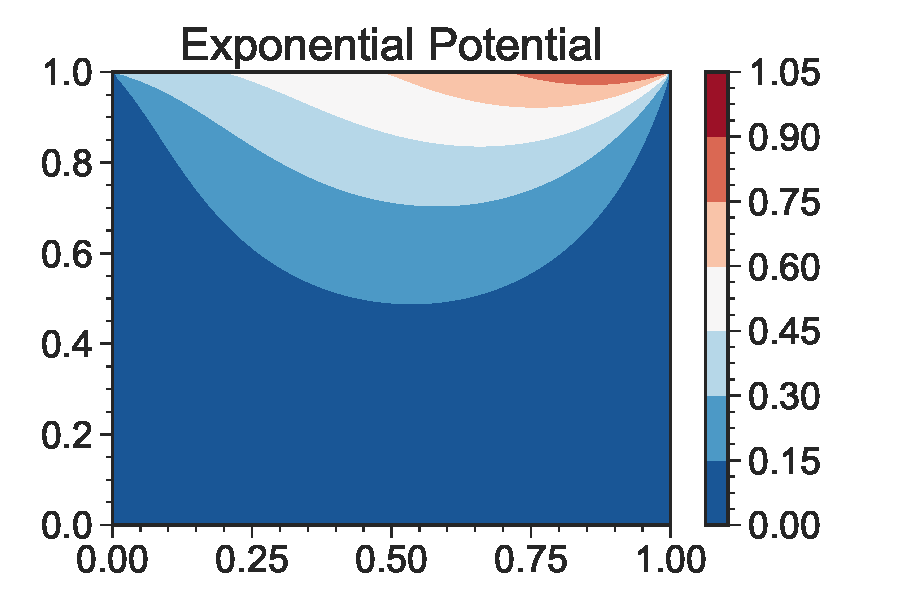
\includegraphics[width=0.3\textwidth]{Images/Fig:Countour-plot/1-contour.pdf}
        }%
        \hspace{1em}
        \subfigure[Contour plot number 2]{%
            \label{fig:Contour_2}
            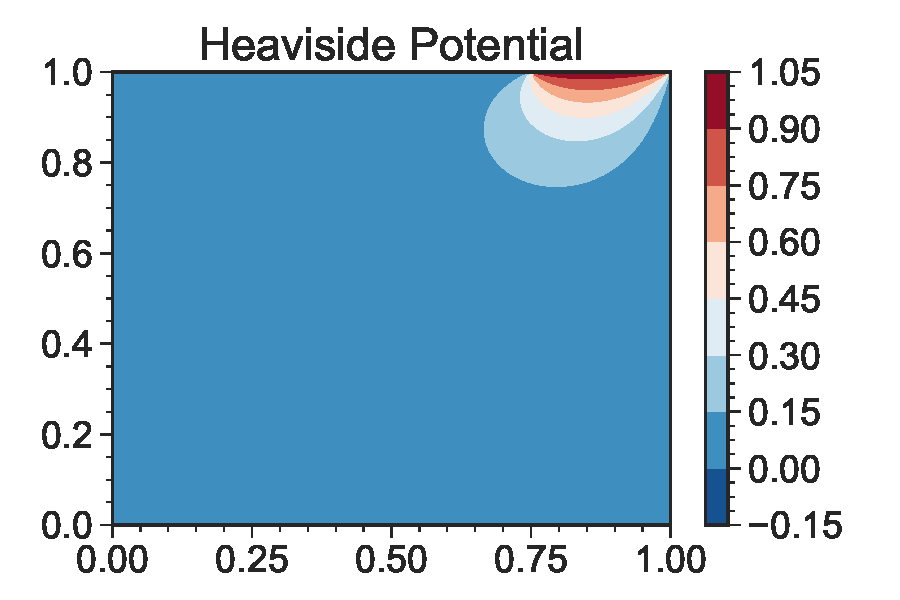
\includegraphics[width=0.3\textwidth]{Images/Fig:Countour-plot/2-contour.pdf}
        }%
        \hspace{1em}
        \subfigure[Contour plot number 3]{%
           \label{fig:Contour_3}
           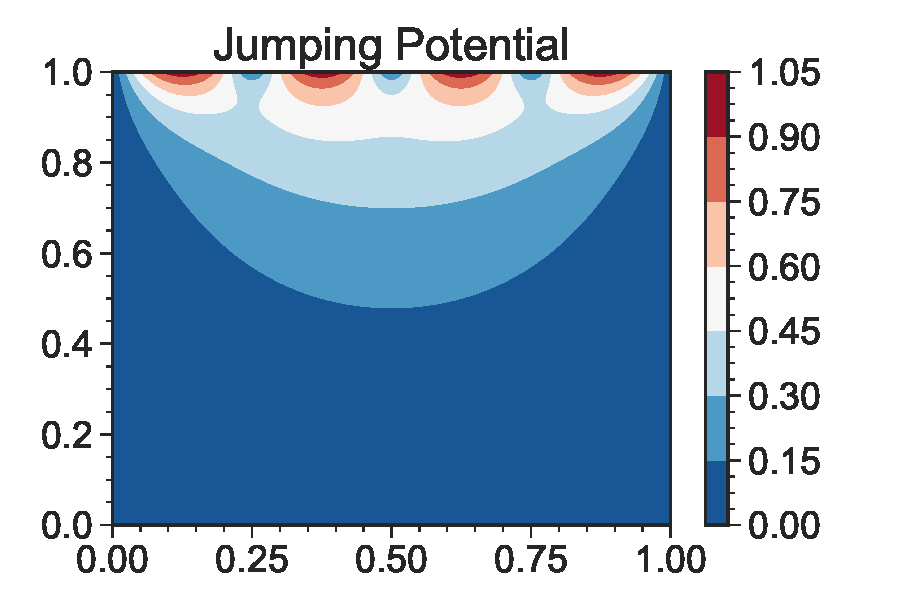
\includegraphics[width=0.3\textwidth]{Images/Fig:Countour-plot/3-contour.pdf}
        }\\ %  ------- End of the first row ----------------------%
        \subfigure[Contour plot number 4]{%
            \label{fig:Contour_4}
            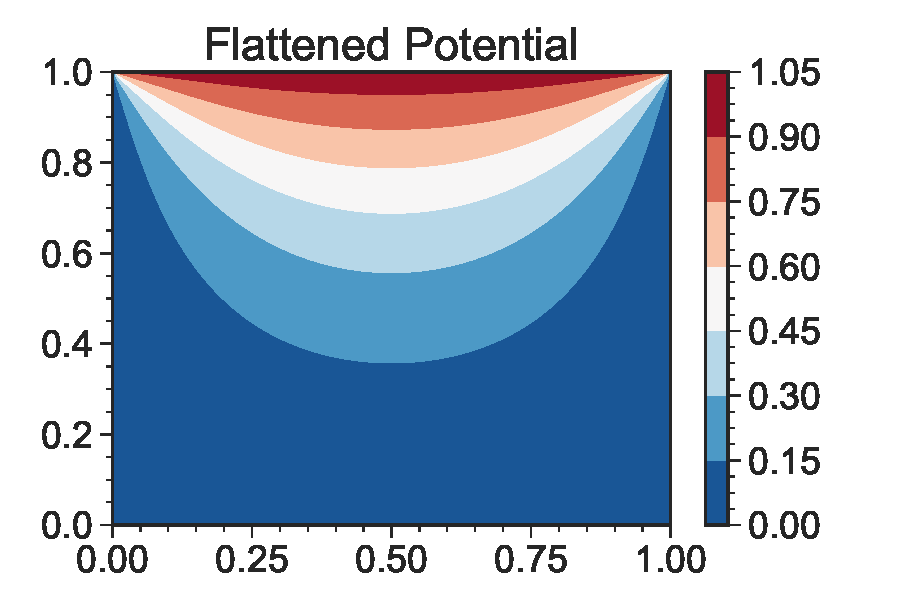
\includegraphics[width=0.3\textwidth]{Images/Fig:Countour-plot/4-contour.pdf}
        }%
        \hspace{1em}
        \subfigure[Contour plot number 5]{%
            \label{fig:Contour_5}
            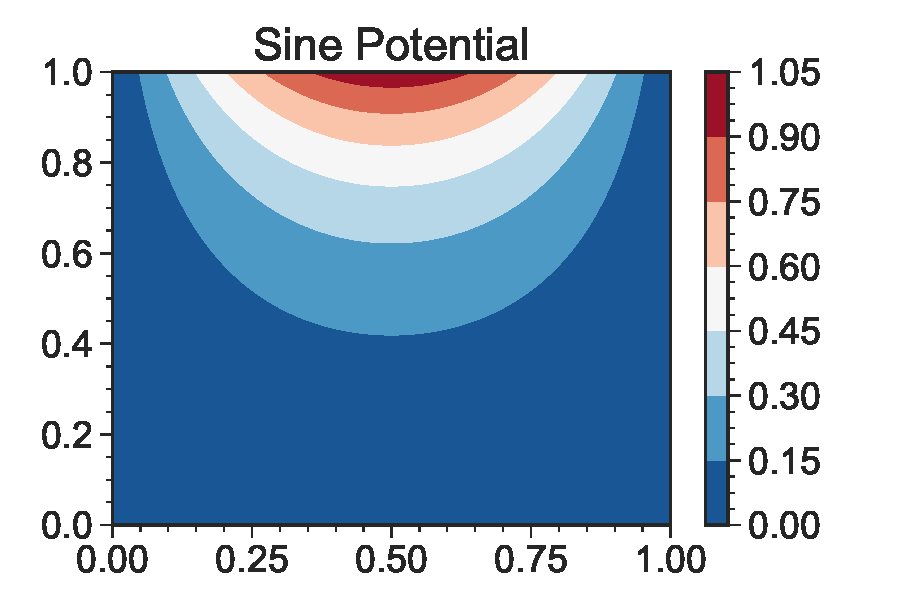
\includegraphics[width=0.3\textwidth]{Images/Fig:Countour-plot/5-contour.pdf}
        }%
        \hspace{1em}
        \subfigure[Contour plot number 6]{%
            \label{fig:Contour_6}
            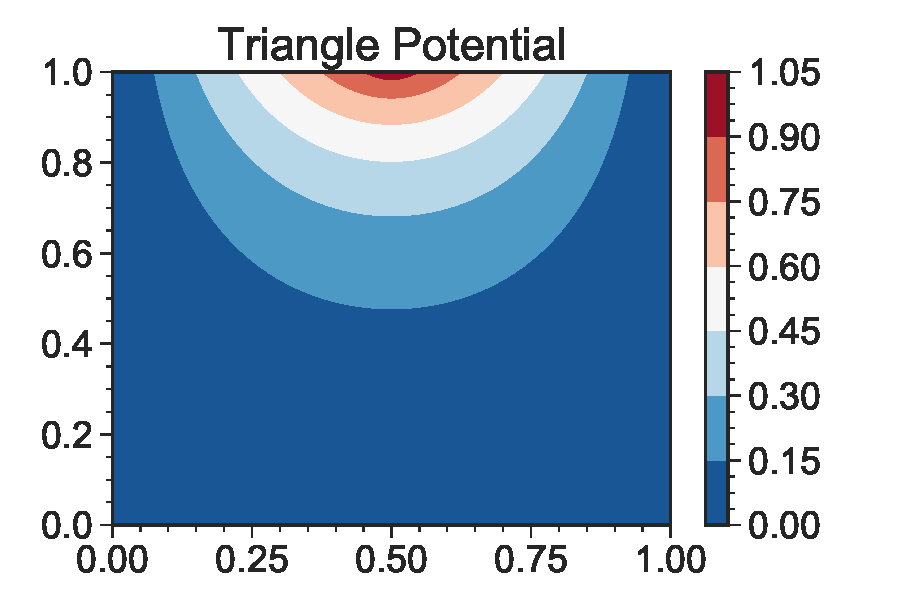
\includegraphics[width=0.3\textwidth]{Images/Fig:Countour-plot/6-contour.pdf}
        }%
%
    \caption{%
        Contour plots for different potentials $V_0(x)$, along the line $y=1$
     }%
   \label{fig:Countour-plot}
\end{figure*} 